%! version 1.0                  <31Dec2017>                      nelson & pedro
% ==============================================================================
% Student Name: Nelson Estevão                           Student Number: A76434
% Student Name: Pedro Ribeiro                            Student Number: A85493
% ------------------------------------------------------------------------------
% Universidade do Minho
% Escola de Engenharia - Departamento de Informática
% Mestrado Integrado em Engenharia Informática
% ------------------------------------------------------------------------------
% Laboratórios de Informática I                           Ano Lectivo 2017/2018
% Micro Machines
% ==============================================================================
\documentclass[a4paper]{report}

% encoding
%-------------------------------------------------------------------------------
\usepackage[utf8]{inputenc}
\usepackage[T1]{fontenc}
%-------------------------------------------------------------------------------

% language
%-------------------------------------------------------------------------------
\usepackage[portuguese]{babel}
%-------------------------------------------------------------------------------

% hyphenation rules
%-------------------------------------------------------------------------------
\usepackage{hyphenat}
\hyphenation{mate-mática recu-perar}
%-------------------------------------------------------------------------------

% figures
%-------------------------------------------------------------------------------
\usepackage{graphicx}
\graphicspath{ {figures/} }
\usepackage{subfig}
%-------------------------------------------------------------------------------

% captions
%-------------------------------------------------------------------------------
\usepackage[font=small,labelfont=bf]{caption}
%\captionsetup{font={small,it}}
%-------------------------------------------------------------------------------

% code snippets
%-------------------------------------------------------------------------------
\usepackage{listings}
\lstset{
  inputencoding=utf8,
  extendedchars=true,
  backgroundcolor=\color{backcolour},
  commentstyle=\color{codegreen},
  keywordstyle=\color{codepurple},
  numberstyle=\tiny\color{codegray},
  stringstyle=\color{magenta},
  basicstyle=\footnotesize,
  breakatwhitespace=false,
  breaklines=true,
  captionpos=b,
  keepspaces=true,
  numbers=none, % options: left, right, none
  numbersep=5pt,
  showspaces=false,
  showstringspaces=false,
  showtabs=false,
  tabsize=2
}
%-------------------------------------------------------------------------------

% colors
%-------------------------------------------------------------------------------
\usepackage{xcolor}
\definecolor{codegreen}{rgb}{0,0.6,0}
\definecolor{codegray}{rgb}{0.5,0.5,0.5}
\definecolor{codepurple}{rgb}{0.58,0,0.82}
\definecolor{backcolour}{rgb}{0.95,0.95,0.95}
%-------------------------------------------------------------------------------

\usepackage[absolute]{textpos}

\title{Relatório Trabalho Prático LI1}
\author{Grupo 138 \\ \\
Nelson Estevão \ \ \ \ \ Pedro Ribeiro}
\date{31 de Dezembro de 2017}
% \date{\today}

\begin{document}

\begin{textblock}{5}(5.5,0)
  \centering
  
\includegraphics[height=5cm]{EEUM_logo}
\end{textblock}

\maketitle

\tableofcontents

\listoffigures

% \listoftables

%_______________________________________________________________________________
%                                                                    Introdução
\chapter{Introdução}

  \section{Contextualização}
  No âmbito da Unidade Curricular de \emph{Laboratórios de Informática I} foi
  requisitado a reprodução de um jogo já existente - ``Micro Machines''. Esta UC
  insere-se no primeiro semestre do plano curricular do Mestrado Integrado em
  Engenharia Informática e serve de complemento prático à Unidade Curricular
  \emph{Programação Funcional}.

  Este projeto foi realizado programando somente na linguagem \emph{Haskell} que
  segue o paradigma funcional. Para realizar a componente gráfica do jogo foi
  usado o Gloss, um pacote presente na biblioteca \emph{open source} do
  Hackage.

  Durante o processo de desenvolvimento foi possível a consulta de um Sistema de
  Feedback criado pelos Docentes da cadeira. Este fornecia informação relativa à
  assertividade das tarefas submetidas a avaliação automática.

  O projeto usou o sistema de controlo de versões, \emph{Subversion (SVN)}, que
  permitiu manter um registo das alterações feitas ao código, assim como,
  facilitar o trabalho em equipa. Além disso, possibilitou o uso de ferramentas
  de apoio como \emph{Hlint}, \emph{HPC} e \emph{Homplexity} que nos davam
  sugestões para tornar o código mais simples e legível, indicavam a percentagem
  e cobertura dos testes e destacavam más práticas de programação,
  respectivamente.

  \section{Motivação}
  De maneira a assimilar conhecimento e melhor entender as possibilidades que a
  programação funcional fornece é vital o desenvolvimento do início ao fim de um
  \emph{software}.

  A possibilidade de o fazer sobre a tutoria dos Docentes torna essa tarefa mais
  acessível. A capacidade de trabalhar em equipa é fulcral e por isso este
  projeto torna-se muito importante para culmatar a falta de experiência do
  grupo.

  \section{Objectivos}
  Durante a realização deste projeto pretende-se familarizar ambos os membros do
  grupo com ferramentas de apoio ao desenvolvimento, o trabalho em equipa usando
  um sistema de controlo de versões centralizado (SVN), fazer a introdução a uma
  \emph{Domain Specific Language} como o \LaTeX \ e aprofundar as competências
  técnicas nesta linguagem de programação em particular que é o \emph{Haskell}.

  Além disso, ter um jogo em funcionamento seria ideal para marcar o projeto
  como terminado.

%_______________________________________________________________________________
%                             Análise de Requisitos e Especificação do Problema
\chapter{Análise de Requisitos}


\section{Fase 1}
\label{sec:analisefase1}

A primeira fase encontrava-se divida em três tarefas. A Tarefa 1 tinha como
objetivo definir a função \texttt{constroi}.

\begin{lstlisting}[language=Haskell]
constroi :: Caminho -> Mapa

type Caminho = [Passo]

data Mapa = Mapa (Posicao,Orientacao) Tabuleiro
\end{lstlisting}

Esta função recebe como único argumento um caminho, i.e. uma lista de passos, e
devolve um mapa.

A Tarefa 2 tinha por finalidade fazer a validação de mapas. A função
\texttt{valida} tem como argumento um mapa e devolve True quando o mapa é válido
e False quando não o é.

\begin{lstlisting}[language=Haskell]
 valida :: Mapa -> Bool
\end{lstlisting}

Esta validação segue determinados critérios pré-estabelecidos, sendo esses:

\begin{itemize}
\item
  Existência de apenas um percurso, à exceção do qual todas as peças são
  do tipo lava.
\item
  O percurso deve ser de natureza tal que partindo de uma peça com uma
  determinada orientação se deva chegar à mesma peça com a mesma orientação.
\item
  A orientação inicial tem de ser compatível com a peça de partida.
\item
  As alturas entre as peças têm de ser compatíveis.
\item
  Todas as peças do tipo lava têm altura 0.
\item
  O mapa é sempre retangular e rodeado por lava, ou seja, a primeira e
  ultima linha, assim como a primeira e última coluna são
  necessariamente constituídas por peças do tipo lava.
\end{itemize}

A Tarefa 3 consistia em criar a função \texttt{movimenta}.

\begin{lstlisting}[language=Haskell]
 movimenta :: Tabuleiro -> Tempo -> Carro -> Maybe Carro
\end{lstlisting}

Esta função recebe um tabuleiro, o tempo de duração do movimento, o carro a
movimentar e devolve \texttt{Nothing} caso tivesse morrido ou então o carro com
a sua posição e vetor atualizado. No cálculo desta posição e vetor teve de ser
tido em conta a mudança de peça e a validade das mesmas, os ricochetes em peças
de altura superior à atual e movimentos inválidos que resultariam na morte do
carro.


\section{Fase 2}
\label{sec:analisefase2}

A segunda fase do projeto foi também dividida em três tarefas. A quarta tarefa
que serve para definir o vetor velocidade do carro. A quinta tarefa é a que
junta todas as fases criando o jogo em si. A sexta consistia em definir um bot
para que ele pudesse tomar decisões num jogo em relação a que ação o carro deve
tomar em cada instante. Além disso, é também nesta fase que o relatório prático
se insere.

A Tarefa 4 traduz-se na elaboração da função \texttt{atualiza} que consiste em
atualizar o estado do jogo consoante uma acção tomada pelo jogador em questão.

\begin{lstlisting}[language=Haskell]
 atualiza :: Tempo -- a duracao da acao
          -> Jogo  -- o estado do jogo
          -> Int   -- o identificador do jogador
          -> Acao  -- a acao tomada pelo jogador
          -> Jogo  -- o estado atualizado do jogo
\end{lstlisting}

Esta função tem de substituir no jogo atual o carro do jogador pelo novo carro
com o seu vetor velcidade atualizado assim como, atualizar as quantidades de
nitro disponivel, assim como o histórico de posições pelas quais cada jogador
passou.

\begin{lstlisting}[language=Haskell]
 data Jogo = Jogo
  { mapa      :: Mapa         -- o mapa do percurso
  , pista     :: Propriedades -- as propriedades do percurso
  , carros    :: [Carro]      -- o estado do carro de cada jogador
  , nitros    :: [Tempo]      -- as quantidades de nitro restantes
  , historico :: [[Posicao]]  -- o historico de posicoes
  }
\end{lstlisting}

No caso de a ação tomada pelo jogador incluir a aplicação de nitro a um outro
jogador que não ele próprio, então o vetor do nitro tem de ser somado ao vetor
velocidade do carro alvo. Isto implica a redução da quantidade de nitro na mesma
do carro do jogador.

A Tarefa 5 foi a tarefa mais livre, em que essencialmente se pretendia a união
de todos as tarefas para a realização do jogo. O desenho dos mapas deve ser
feito com o auxílio da Tarefa 1 e a validação dos mesmos com auxílio da Tarefa 2.
Aqui entra a biblioteca Gloss para a criação da componente gráfica uma vez que
esta nos fornece os tipo de dados \texttt{Picture} e \texttt{Event}.

A Tarefa 6 tinha como objetivo a criação de regras que faziam a tomada de
decisão um bot. Assim, para cada instante este devia decidir se devia acelerar,
travar, virar à esquerda, virar à direita, aplicar nitro a si ou a um oponente.

\begin{lstlisting}[language=Haskell]
 bot :: Tempo  --  tempo decorrido desde a ultima decisao
     -> Jogo   --  estado atual do jogo
     -> Int    --  identificador do jogador dentro do estado
     -> Acao   --  a decisao tomada pelo bot
\end{lstlisting}

O propósito do bot era participar num torneio com os restantes grupos de modo a
concluir quais obtinham melhores resultados. O torneio pretendia ter várias
fases onde ganharia o bot que desse primeiro uma volta ou então no fim de 60
segundos, aquele que estivesse mais próximo. Cada jogador tinha direito a 5
segundos de nitro.


%_______________________________________________________________________________
%                                             Descrição da Solução Desenvolvida
\chapter{A Nossa Solução}
\label{sec:solucao}

Na Tarefa 1 começamos por contruir um tabuleiro com as mesmas dimensões do
caminho dado com somente com \texttt{Peca Lava 0}.

\begin{lstlisting}[language=Haskell]
 constroiTabuleiroBase :: Caminho -> Tabuleiro
\end{lstlisting}

Para isso usamos a função \texttt{dimensao}, definida pelos docentes, que nos dava
um par com a dimensão do tabuleiro para aquele caminho. Após contruir um
tabuleiro com essa dimensão, fomos substituindo as peças de lava pela a peça
imposta pelo caminho. Para isso foi preciso definir funções auxiliares que
tivessem em conta a altura das peças anteriores, a posição anterior e a
orientação.

Para validar os mapas gerados por caminhos, começamos por definir funções que
verificassem se cada uma das condições enunciadas na Secção
\ref{sec:analisefase1} eram respeitadas. Após isso, usamos a função final para
unir essas funções e descobrir se era ou não válido.

\begin{lstlisting}[language=Haskell]
 valida :: Mapa -> Bool
 valida (Mapa (p,o) tb) = a && b && c && d && e
                      where
                        a = orientacaoFstPeca (Mapa (p,o) tb)
                        b = periferiaLava tb
                        c = testaLava tb
                        d = testaPercurso (Mapa (p,o) tb)
                        e = verificaNotPercurso (Mapa (p,o) tb)
\end{lstlisting}

Na Tarefa 3 começamos por definir os casos em que o carro não morre. Desta
maneira conseguimos perceber que todos os casos restantes o carro morre e por
isso, a função movimenta deve retornar \texttt{Nothing}. Posto isto, tentamos
definir o caso mais simples em que não existe colisões que resultem em
ricochete, onde o movimento é linear, e devolver antes um carro em que a posição
foi correctamente alterada assim como o vetor velocidade possa ou não ter sido
alterado para refletir a mudança de direção do carro.

A Tarefa 4 tem o papel importante de definir o vetor velocidade consoante a ação
do jogador. Começamos por definir os vetores de todas as forças que atuam sobre
o carro separadamente. Com estas função definidas somavamos primeiro ao vetor
velocidade as forças da aceleração, do atrito, dos pneus e quando estava numa
rampa o vetor da gravidade. Nesse mesmo momento, a direção também era atualizada
quando o jogador estivesse a virar. Só depois disso é que aplicamos o vetor
nitro no caso de a ação do jogador assim o fizer. O vetor nitro é aplicado no
carro alvo, mas o tempo do histórico de nitro restante é retirado ao carro do
jogador. Nesta tarefa, uma vez que se tinha de atualizar todo o jogo, é também
atualizado o histórico de posições onde se acrescenta a posição atual à lista
caso esta ainda lá não esteja.

Na Tarefa 5 estabelecemos que iríamos definir a dimensão da janela do jogo como
(1000,1000) (pixeis). Deste modo, sabendo que as nossas imagens são quadradas e
têm 600 pixeis de lado, o próximo passo era definir um fator de scaling para as
imagens tendo em conta a dimensão do mapa que pretendemos desenhar.

Para conseguirmos desenhar um mapa precisamos de saber para que posições da
janela devem ir as peças, trabalho desempenhado pela função
\texttt{windowPositions}. Deste modo faltava associar peças a figuras, função
desempenhada pela função \texttt{pecaToPicture}. Deste modo, de forma sucinta, o
desenho de cada estado fica a cargo da função \texttt{drawState}.

\begin{figure}[h]
\label{fig:estado}
\centering
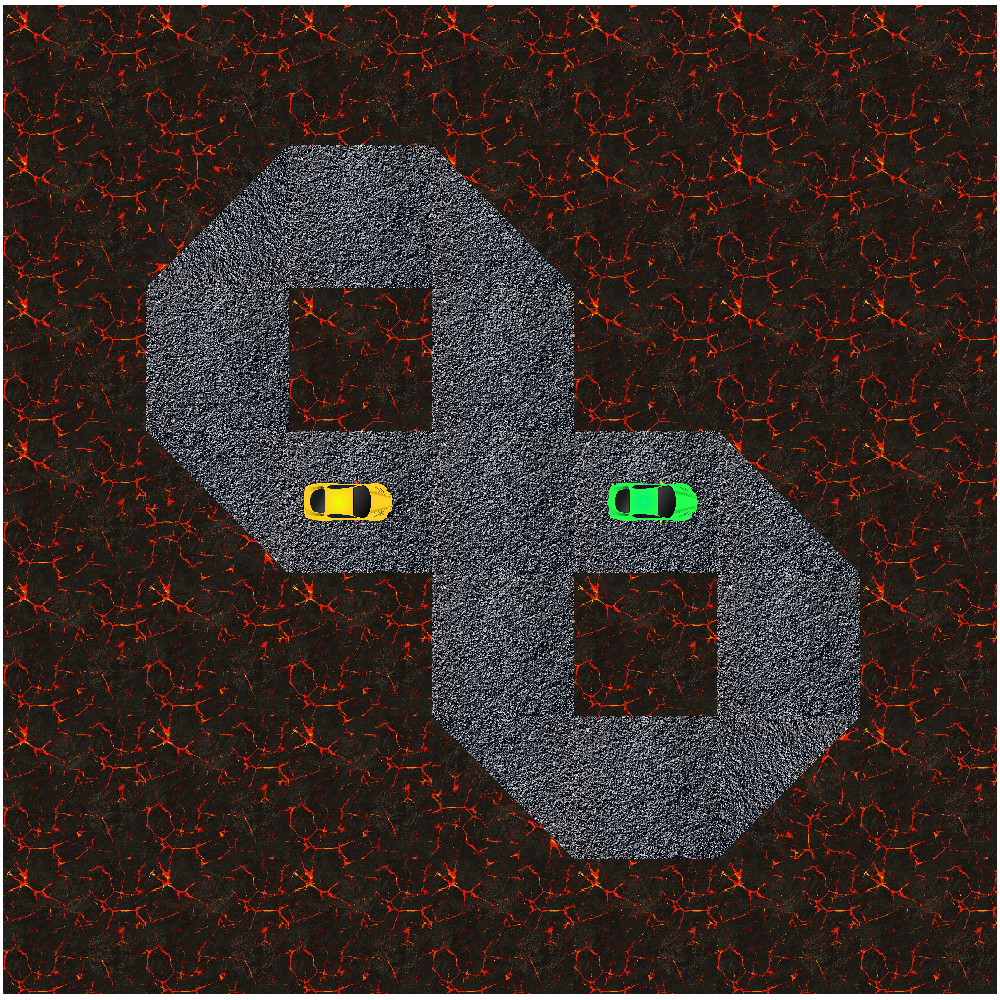
\includegraphics[width=8cm]{exemplo-mapa}
\caption{Exemplo de um estado do jogo.}
\end{figure}

Cada estado é constituído por uma lista de jogos, uma lista de imagens, uma
lista de ações, um bool e um inteiro. A lista de jogos contém os jogos
correspondentes aos quatros mapas do jogo em cada instante, as imagens são todas
as que foram carregadas em \texttt{main}, a lista de ações é constituída pela ação do
carro 1 e do carro 2 ou pela ação do carro 1 e ação do bot,
respetivamente. O bool é \texttt{False} caso a corrida ainda não tenha acabado e
\texttt{True} caso contrário. O inteiro identifica em que estado do jogo nos
encontramos.


Na Tarefa 6 para tentarmos alcançar o melhor resultado possível tentamos seguir
a seguinte estratégia:

\begin{itemize}
\item
  A base da estratégia é considerar a peça em que se está e a peça que
  vem a seguir.
\item
  Assim o bot analisa a peça em que se encontra e verifica a necessidade
  de virar para conseguir obter a direção necessária para que possa
  entrar corretamente na próxima peça.
\item
  A estratégia relativa à utilização de nitros passa essencialmente por
  verificar se o concorrente que se encontra mais próximo do nosso carro
  se encontra numa peça do tipo curva com altura superior ou igual a 0.
  Caso a condição anterior se verifique então aplicamos nitro ao
  concorrente, caso contrário apenas continuamos a marcha. Achamos
  pertinente incluir a claúsula relativa à altura porque na maioria dos
  casos se aplicassemos nitro a concorrente em peças do tipo curva com
  altura menor que 1 estes iriam ser ajudados ao invés de serem
  prejudicados em consequência das colisões que se verificam em peças
  com altura inferior a 0.
\end{itemize}



%_______________________________________________________________________________
%                                                          Validação da Solução
\chapter{Validação da Solução}

Durante todo o desenvolvimento o ghci tornou-se de extrema relevância para
atestar o correcto funcionamento do nosso código. Em primeiro lugar, por
verificar a cada vez tentamos interpretar o nosso código, o ghci nos dar
mensagens de erro que impedem a construção de mais código por cima de funções
implementadas de forma incorreta.

Em cada tarefa contamos com o auxílio do sistema de \emph{feedback} que para
as primeiras quatro tarefas existia a possibilidade de comparar através de
testes definidos por nós os nossos resultados com os dos Docentes. Isto foi a
parte fulcral para o sucesso dessas tarefas visto que muitos resultados que ao
início poderiamos considerar corretos diferenciavam de alguma forma. Durante
o desenvolvimento, foram sempre sendo pequenos testes feitos a cada função que
era escrita e avaliado individualmente se o \emph{output} faria sentido.

A validação da tarefa 5 teve duas fases: uma fase mais empírica e outra mais
analítica. Tivemos uma primeira fase em que verificamos se os mapas estavam
realmente bem desenhados, ou seja, se aparecia na janela do jogo aquilo que
realmente estavamos à espera. Após testes com vários mapa achamos que estamos em
condições de validar o método que tínhamos criado para a construção das imagens
do jogo. Passada esta parte tivemos de validar uma função fulcral desta tarefa -
a função \texttt{atualizaMovimenta} que recebe um novo jogo a cada frame de
acordo com a Tarefa 4 e atualiza a posição do carro de acordo com a Tarefa 3.
Fizemos testes com esta função e achamos estar em condições de a validar. É
pertinente referir que esta função não produz resultados integralmente
verdadeiros devido ao facto de a Tarefa 3 não estar completa e não considerar
todos os casos possíveis. Assim fazemos uma validação consciente desta tarefa,
reconhecendo que os mapas assim como os carros estão a ser bem desenhados embora
a sua posição não esteja a ser atualizada com a maior correção.

No que à Tarefa 6 diz respeito, verificamos que o nosso bot tem a capacidade de
fazer qualquer percurso do início ao fim. No entanto, existem percursos em que
as propriedades do jogo implicam um maior número de mortes o que nos dá uma
pior prestação nessas pistas. Ainda assim, os nossos resultados nos torneiros
indicavam uma posição favorável em relação à média dos restantes grupos.

%_______________________________________________________________________________
%                                                                     Conclusão
\chapter{Conclusão}

De um modo geral, este trabalho foi enriquecedor para ambos os membros do grupo.
Consideramos que teve um impacto positivo na nossa aprendizagem na programação
de programas. As nossas capacidades e conhecimentos em relação à linguagem
\emph{Haskell} aumentaram e foram aprofundadas.

O desafio teve um acréscimo de valor enorme naquilo que era a reduzida
experiência deste grupo. Adquirimos conhecimentos a nível de desenvolvimento
de \emph{software}, de como corretamente armazenar o nosso código e percebemos a
importância de trabalhar em equipa para atingir objetivos maiores.

O nosso nível de satisfação com o resultado do projeto é positivo. No entanto,
sentimos que pode ser considerado um trabalho inacabado, o que gostariamos de
ter conseguido no prazo estipulado não sentir. Gostariamos no futuro de repetir
a experiência e terminar este jogo.


% \bibliographystyle{plain}
% \bibliography{document}

\end{document}
\grid
